\begin{figure}[htbp]
\centering 
  \subfloat[Box plot \acs{SCT}.]{
	  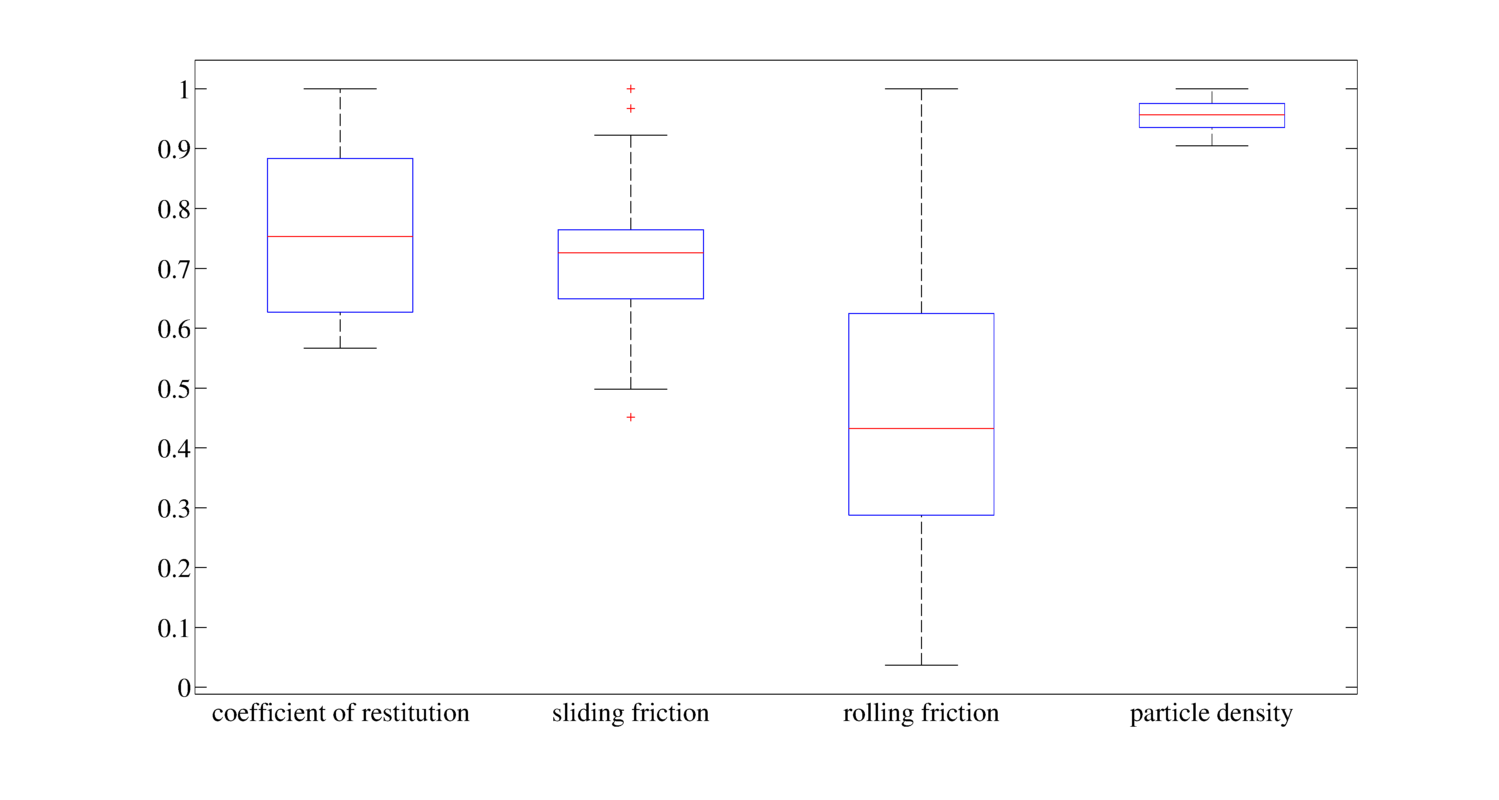
\includegraphics[width=.47\columnwidth]{images/167BoxSCTcokefinetest02coeffP1}
	  \label{fig:167BoxSCTcokefinetest02coeffP1}
  }
  \quad
  \subfloat[Density plot \acs{SCT}.]{
	  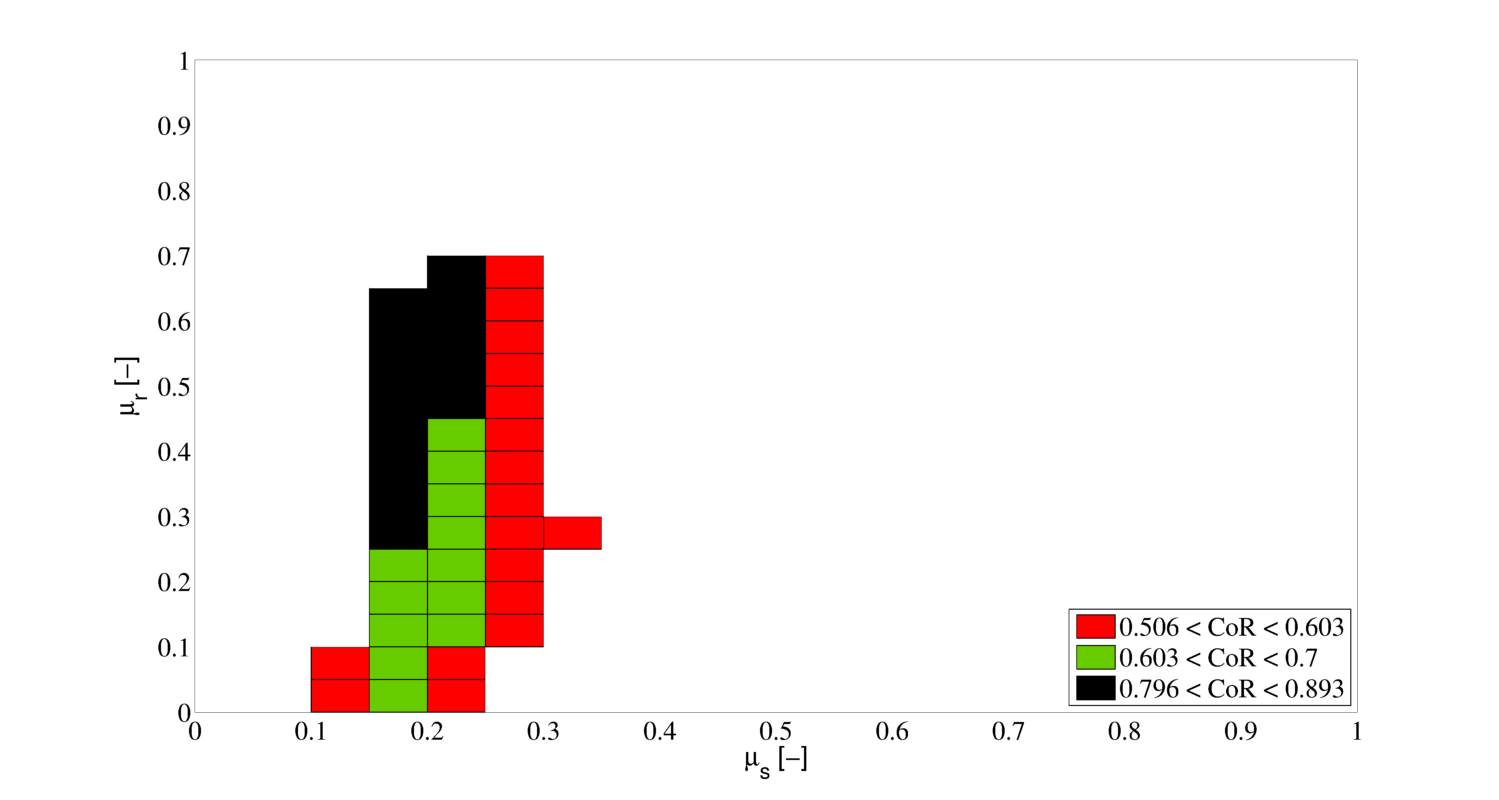
\includegraphics[width=.47\columnwidth]{images/173TileSCcokefinetest02coeffP1-2}
	  \label{fig:173TileSCcokefinetest02coeffP1-2}
  }
  \\  
  \subfloat[Box plot \acs{AoR}.]{
	  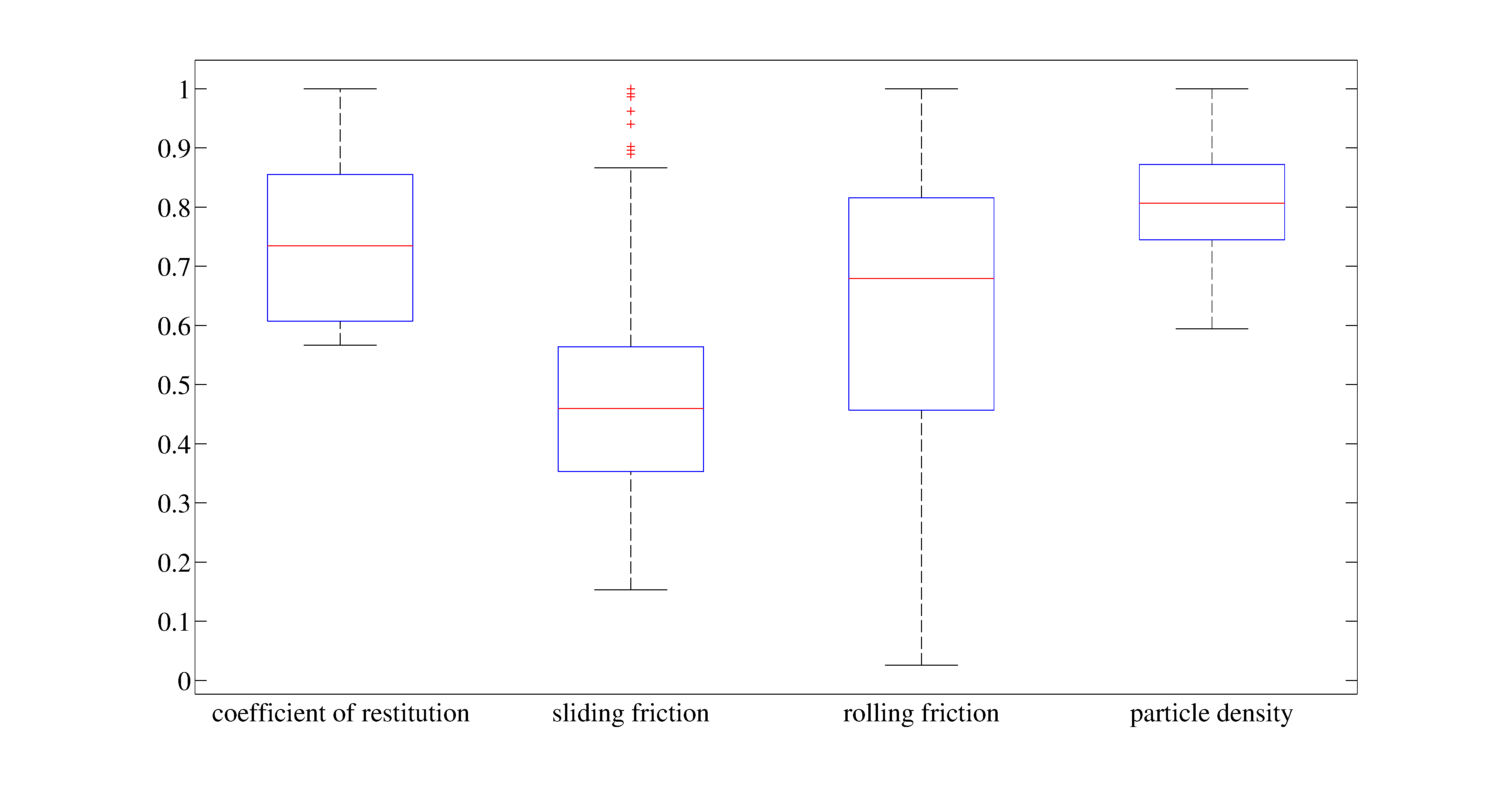
\includegraphics[width=.47\columnwidth]{images/179BoxAORcokefine}
	  \label{fig:179BoxAORcokefine}  }
  \quad
  \subfloat[Density plot \acs{AoR}.]{
	  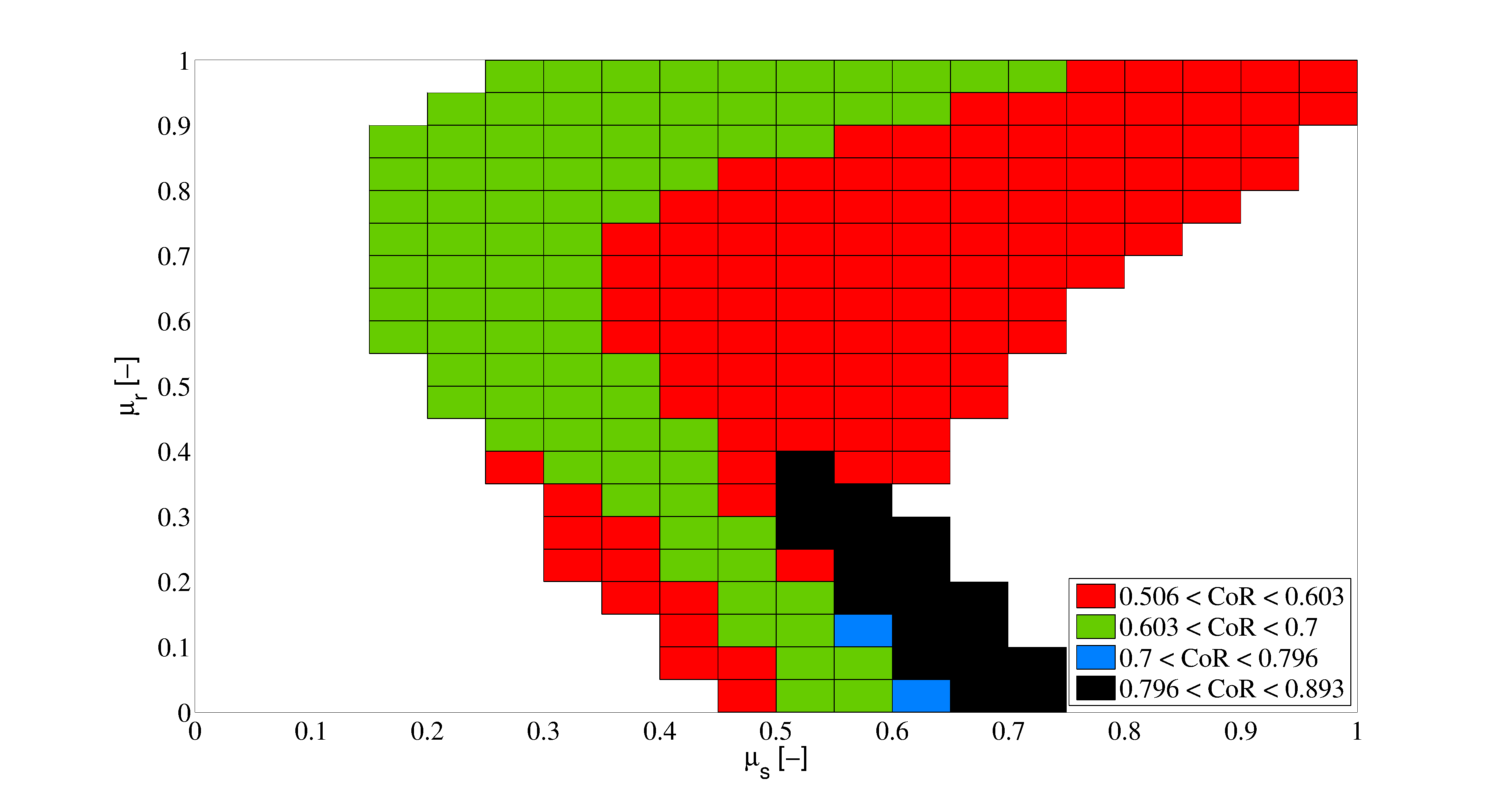
\includegraphics[width=.47\columnwidth]{images/180TileAORcokefine}
	  \label{fig:180TileAORcokefine}  }
  \\  
  \subfloat[Box plot intersection: \acs{AoR} \& \acs{SCT}.]{
	  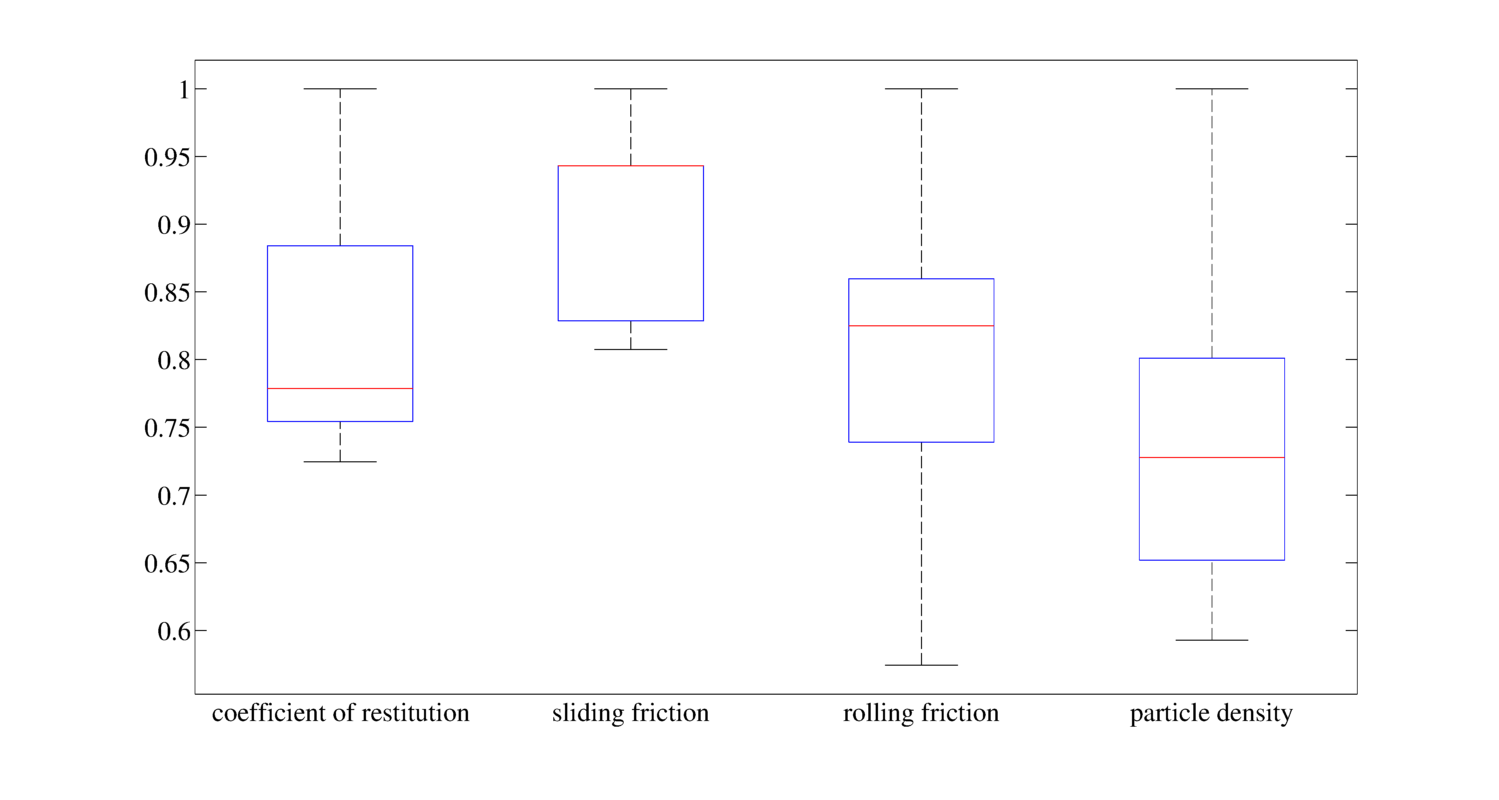
\includegraphics[width=.47\columnwidth]{images/191BoxMixcokefine_3}
	  \label{fig:191BoxMixcokefine_3}
  }
  \quad
  \subfloat[Density plot intersection: \acs{AoR} \& \acs{SCT}.]{
	  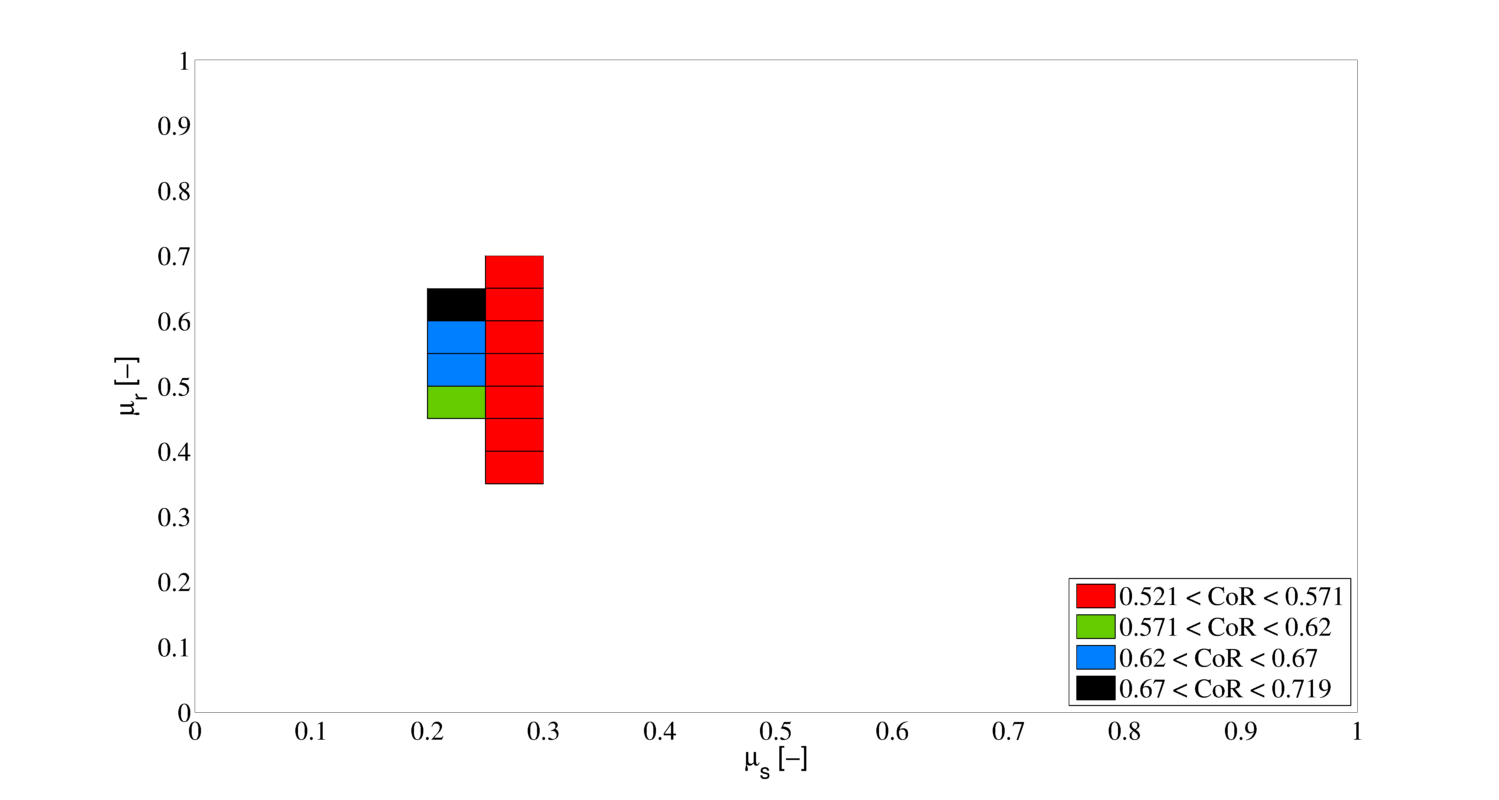
\includegraphics[width=.47\columnwidth]{images/192TileMixcokefine_3}
	  \label{fig:192TileMixcokefine_3}
  }
  \\     
  \caption[Coke fine valid values]{Coke fine valid values. The valid values for the \acs{SCT} and
  \acs{AoR} tests are shown, together with the merge values, valid for both.
  The plots referring to the single test show reasonably narrow confidence
  ranges, while Fig. \ref{fig:191BoxMixcokefine_3} shows unreasonably large
  valid ranges. See Section \ref{sec:remainingmaterialscharacterization} for
  the interpretation.}
  \label{fig:211boxplotscokefine}
\end{figure}